\chapterimage{chapter-t2-bg} % Chapter heading image

\chapter{Configuration}

Most of Stellarium's configuration is done using the configuration
window and the view window. To open the configuration window, click the
button on the left side toolbar or press F2. To open the view window
click the button on the left side toolbar or press F4.

Some options may only be configured by editing the configuration file.
See \href{Advanced_Use\#The_Main_Configuration_File}{ configuration
file} for more details.

\section{Setting the Date and Time}\label{setting-the-date-and-time}

\begin{figure}[h]
\centering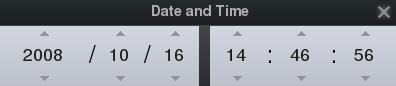
\includegraphics{date_and_time_dialog}
%\caption{Figure caption}
\end{figure}

In addition to the time rate control buttons on the main toolbar, you
can use the date and time window to set the simulation time. The values
for year, month, day, hour, minutes and seconds may be modified by
typing new values, by clicking the up and down arrows above and below
the values, and by using the mouse wheel.

\section{Setting Your Location}\label{setting-your-location}

\begin{figure}[h]
\centering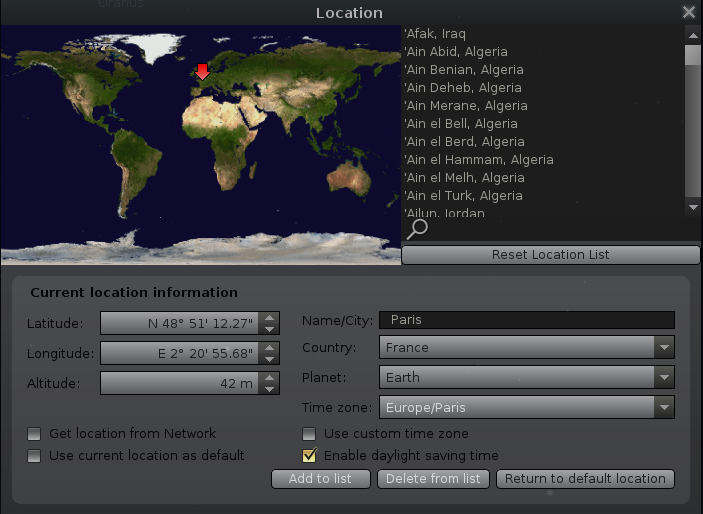
\includegraphics[scale=0.68]{location_dialog}
%\caption{Figure caption}
\end{figure}

The positions of the stars in the sky is dependent on your location on
Earth (or other planet) as well as the time and date. For Stellarium to
show accurately what is (or will be/was) in the sky, you must tell it
where you are. You only need to do this once - Stellarium can save your
location so you won't need to set it again until you move.

To set your location, press F6 to open the location window. There are a
few ways you can set your location:

\begin{enumerate}
\item
  Just click on the map.
\item
  Search for a city where you live using the search edit box at the top
  right of the window, and select the right city from the list.
\item
  Enter a new location using the longitude, latitude and other data.
\end{enumerate}

Once you're happy that the location is set correctly, click on the ``use
as default'' checkbox, and close the location window.

\subsection{The Configuration Window}\label{the-configuration-window}

The configuration window contains general program settings, and many
other settings which do not concern specific display options.

\begin{figure}[h]
\centering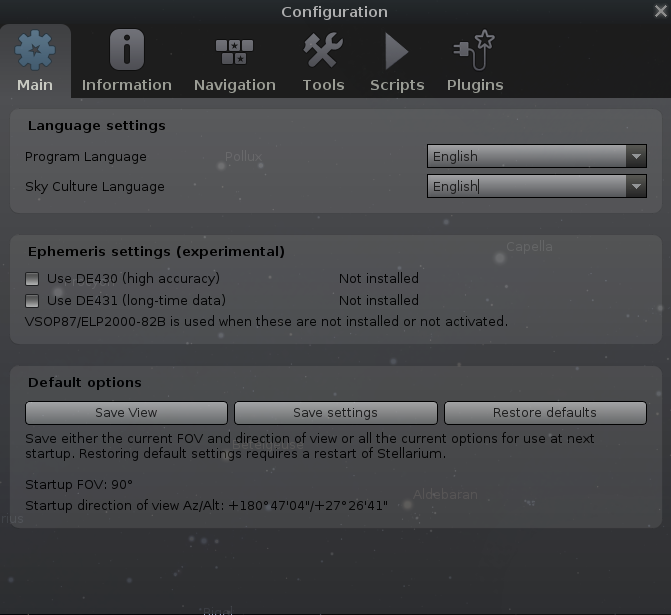
\includegraphics[scale=0.68]{config_dialog_main_tab}
%\caption{Figure caption}
\end{figure}

The Main tab in the configuration window provides controls for changing
the program language, how much information is shown about selected sky
objects, and provides a button for saving the current program
configuration.

\begin{figure}[h]
\centering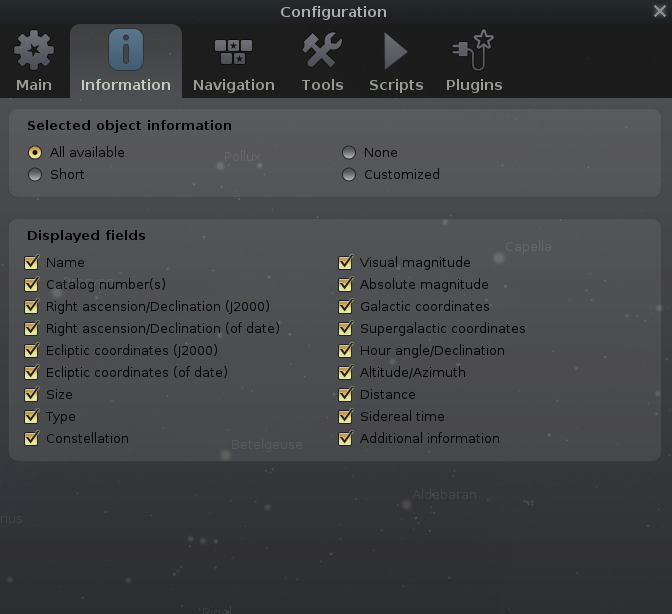
\includegraphics[scale=0.68]{config_dialog_info_tab}
%\caption{Figure caption}
\end{figure}

The Information tab allows you to set the type and amount of information
displayed on a selected object.
\begin{itemize}
\item Ticking or unticking the relevant boxes will control this.
\item The information displays in various colours depending on the type and
level of the stored data
\end{itemize}

\begin{figure}[h]
\centering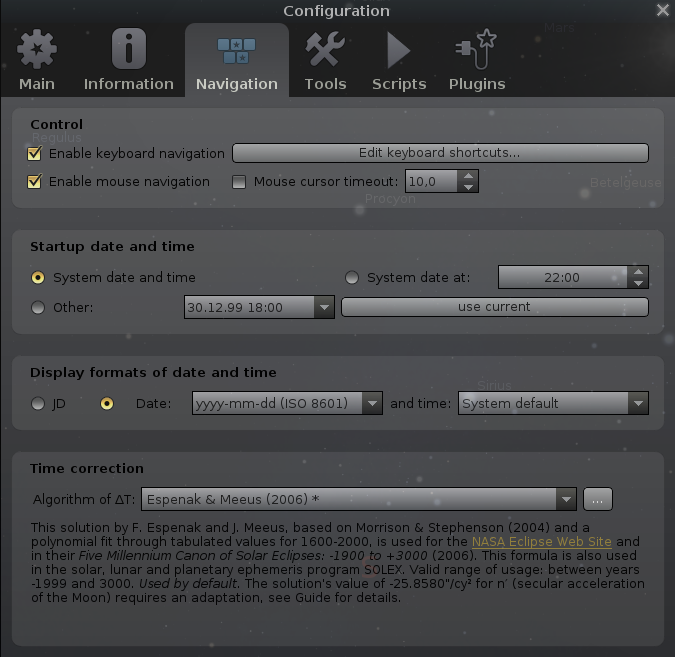
\includegraphics[scale=0.68]{config_dialog_navigation_tab}
%\caption{Figure caption}
\end{figure}

The Navigation tab allows for enabling/disabling of keyboard shortcuts
for panning and zooming the main view, and also how to specify what
simulation time should be used when the program starts:

\begin{itemize}
\item
  When ``Syetem date and time'' is selected, Stellarium will start with
  the simulation time equal to the operating system clock.
\item
  When ``System date at'' is selected, Stellarium will start with the
  same date as the operating system clock, but the time will be fixed at
  the specified value. This is a useful setting for those people who use
  Stellarium during the day to plan observing sessions for the upcoming
  evening.
\item
  When ``Other'' is selected, some fixed time can be chosen which will
  be used every time Stellarium starts.
\end{itemize}

\begin{figure}[h]
\centering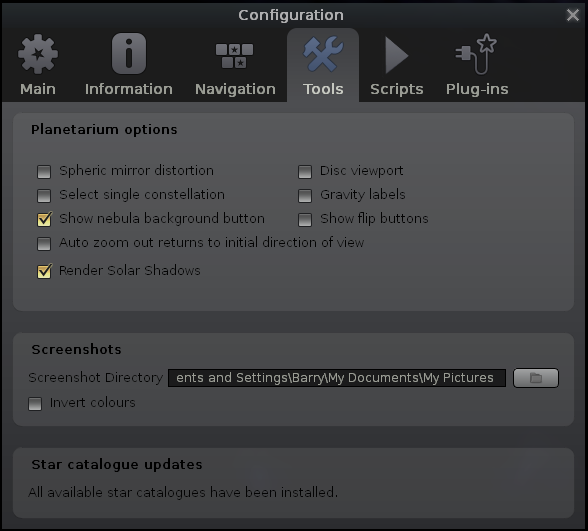
\includegraphics[scale=0.68]{config_dialog_tools_tab}
%\caption{Figure caption}
\end{figure}

The Tools tab of the configuration window contains miscellaneous utility
features:

\begin{itemize}
\item
  \textbf{Show flip buttons} When enabled, two buttons will be added to
  the main tool-bar which allow the main view to be mirrored in the
  vertical and horizontal directions. This is useful when observing
  through telecopes which may cause the image to be mirrored.
\item
  \textbf{Spheric mirror distortion} This option pre-warps the main view
  such that it may be projected onto a spherical mirror using a
  projector. The resulting image will be refected up from the spherical
  mirror in such a way that it may be shone onto a small planetarium
  dome, making a cheap planetarium projection system.
\item
  \textbf{Disc viewport} This option limits masks the main view
  producing the effect of a telescope eyepiece. It is also useful when
  projecting Stellarium's output with a fish-eye lens planetarium
  projector.
\item
  \textbf{Gravity labels} This option makes labels of objects in the
  main view align with the nearest horizon. This means that labels
  projected onto a dome are always alighned properly.
\item
  \textbf{Auto zoom out returns to initial field of view} When enabled,
  this option changes the behaviour of the zoom out key
  (\textbackslash{}) so that it resets the initial direction of view in
  addition to the field of view.
\end{itemize}

\begin{figure}[h]
\centering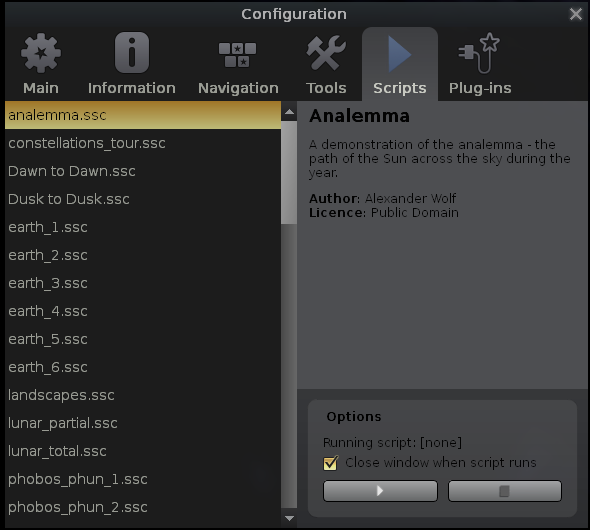
\includegraphics[scale=0.68]{config_dialog_scripts_tab}
%\caption{Figure caption}
\end{figure}

The Scripts tab allows the selection of pre-assembled scripts bundled
with stellarium that can be run. This list can be expanded in your user
area with your own scripts as required.:

• When a scipt is selected it can be run by pressing the arrow button
and stopped with the stop button. With some scripts the stop button is
inhibited until the script is finished.

• Scripts that use sound will need a version of stellarium compiled at
compile time with sound enabled. It must be pointed out here that sound
when enabled depends on the sound capabilities of you computer plarform
and may not work..

• Scripts that contain Video clips will need a suitable video player
that enabled on tour computer..

\begin{figure}[h]
\centering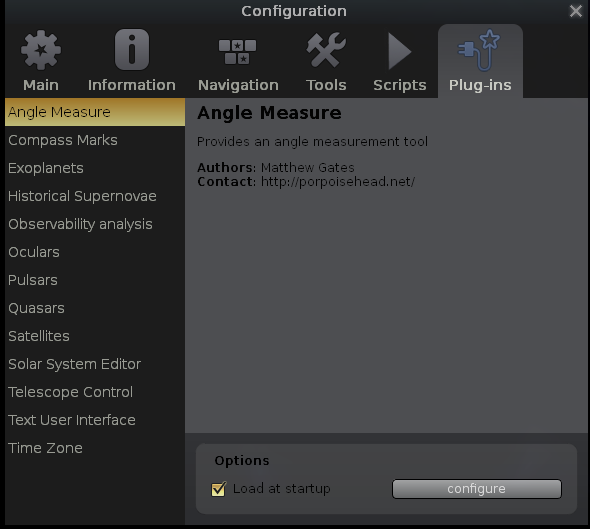
\includegraphics[scale=0.68]{config_dialog_plugins_tab}
%\caption{Figure caption}
\end{figure}

The Plugins tab. Plug ins need to be enabled at start up to be available
as shown on the bar. This allows for the selection of the plugins that
you wish to be enabled at this time:

\section{The View Settings Window}\label{the-view-settings-window}

The View settings window controls many display features of Stellarium
which are not available via the main toolbar.

\subsection{Sky Tab}\label{sky-tab}

\begin{figure}[h]
\centering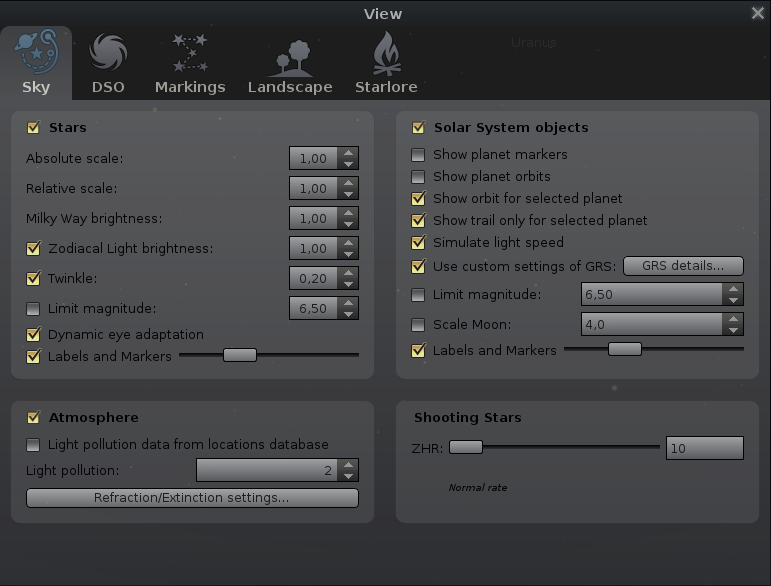
\includegraphics[scale=0.68]{view_dialog_sky_tab}
%\caption{Figure caption}
\end{figure}

The Sky tab of the View window{[}fig:viewwinskytab{]} contains settings
for changing the general appearane of the main sky view. Some
hightlights:

\begin{itemize}
\item
  \textbf{Absolute scale} is the size of stars as rendered by
  Stellarium. If you increase this value, all stars will appear larger
  than before.
\item
  \textbf{Relative scale} determines the difference in size of bright
  stars compared to faint stars. Values higher than 1.00 will make the
  brightest stars appear much larger than they do in the sky. This is
  useful for creating star charts, or when learning the basic
  constellations.
\item
  \textbf{Twinkle} controls how much the stars twinkle.
\item
  \textbf{Dynamic eye adaptation} When enabled this feature reduces the
  brightness of faint objects when a bright object is in the field of
  view. This simulates how the eye can be dazzled by a bright object
  such as the moon, making it harder to see faint stars and galaxies.
\item
  \textbf{Light pollution} In urban and suburban areas, the sky is
  brightned by terrestrial light pollution reflected in the atmophere.
  Stellarium simulates light pollution and is calibrated to the
  \emph{Bortle Dark Sky Scale} where 1 means a good dark sky, and 9 is a
  very badly light-polluted sky. See
  \href{Advanced_Use\#Light_Pollution}{Light Pollution} for more
  information.
\item
  \textbf{Planets and satellites} this group of options lets you turn on
  and off various features related to the planets. Simulation of light
  speed will give more precise positions for planetary bodies which move
  rapidly against backround stars (e.g. the moons of Jupiter). The
  \emph{Scale Moon} option will increase the apparent size of the moon
  in the sky, which can be nice for wide field of view shots.
\item
  \textbf{Labels and markers} you can independantly change the amount of
  labels displayed for planets, stars and nebuulae. The further to the
  right the sliders are set, the more labels you will see. Note that
  more labels will also appear as you zoom in.
\item
  \textbf{Shooting stars} Stellarium has a simple meteor simulation
  option. This setting controls how many shooting stars will be shown.
  Note that shooting stars are only visible when the time rate is 1, and
  might not be visiable at some times of day. Meteor showers are not
  currently simulated.
\end{itemize}

\subsection{Marking Tab}\label{marking-tab}

\begin{figure}[h]
\centering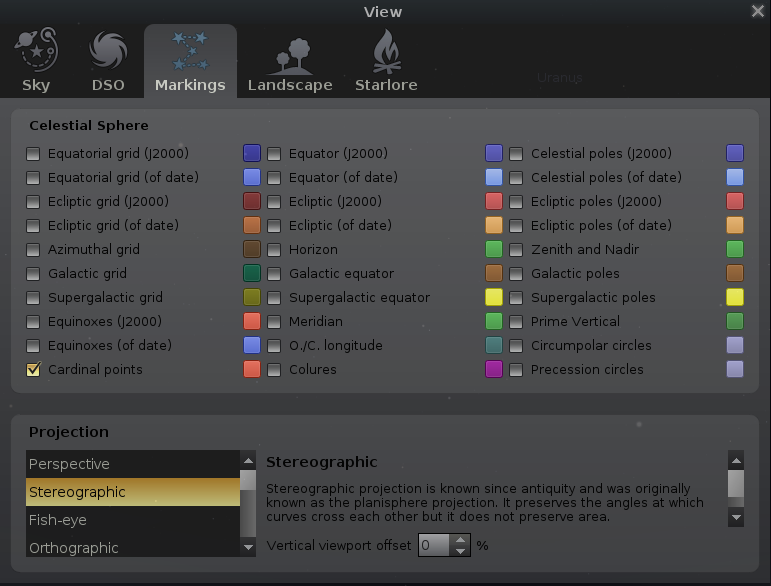
\includegraphics[scale=0.68]{view_dialog_markings_tab}
%\caption{Figure caption}
\end{figure}

The Markings tab of the View window controls the following features:

\begin{itemize}
\item
  \textbf{Celestial sphere} this group of options makes it possible to
  plot various grids and lines in the main view.
\item
  \textbf{Constellations} these controls let you turn on and off
  constellation lines, names, art and boundaries, and control the
  brightness of the constellation artwork.
\item
  \textbf{Projection} Selecting items in this list changes the
  projection method which Stellarium uses to draw the sky. Options are:

  \begin{itemize}
  \item
    \textbf{cylinder} The full name of this projection mode is
    \emph{cylindrical equidistant projection}. The maximum field of view
    in this mode is 233\degree.
  \item
    \textbf{equal area} The full name of this projection method is,
    \emph{Lambert azimuthal equal-area projection}. The maximum field of
    view is 360\degree.
  \item
    \textbf{fish-eye} Stellarium draws the sky using \emph{azimuthal
    equidistant projection}. In fish-eye projection, straight lines
    become curves when they appear a large angular distance from the
    centre of the field of view (like the distortions seen with very
    wide angle camera lenses). This is more pronounced as the user zooms
    out. The maximum field of view in this mode is 180\degree.
  \item
    \textbf{Hammer-Aitoff} The Hammer projection is an equal-area map
    projection, described by Ernst Hammer in 1892 and directly inspired
    by the Aitoff projection. The maximum field of view in this mode is
    360\degree.
  \item
    \textbf{mercator} Mercator projection preserves the angles between
    objects, and the scale around an object the same in all directions.
    The maximum field of view in this mode is 233\degree.
  \item
    \textbf{orthographic} Orthographic projection is related to
    perspective projection, but the \emph{point of perspective} is set
    to an infinite distance. The maximum field of view is 180\degree.
  \item
    \textbf{perspective} Perspective projection keeps the horizon a
    straight line. The maximum field of view is 150\degree. The mathematical
    name for this projection method is \emph{gnomonic projection}.
  \item
    \textbf{stereographic} This mode is similar to fish-eye projection
    mode. The maximum field of view in this mode is 235\degree.
  \end{itemize}
\end{itemize}

\subsection{Landscape Tab}\label{landscape-tab}

\begin{figure}[h]
\centering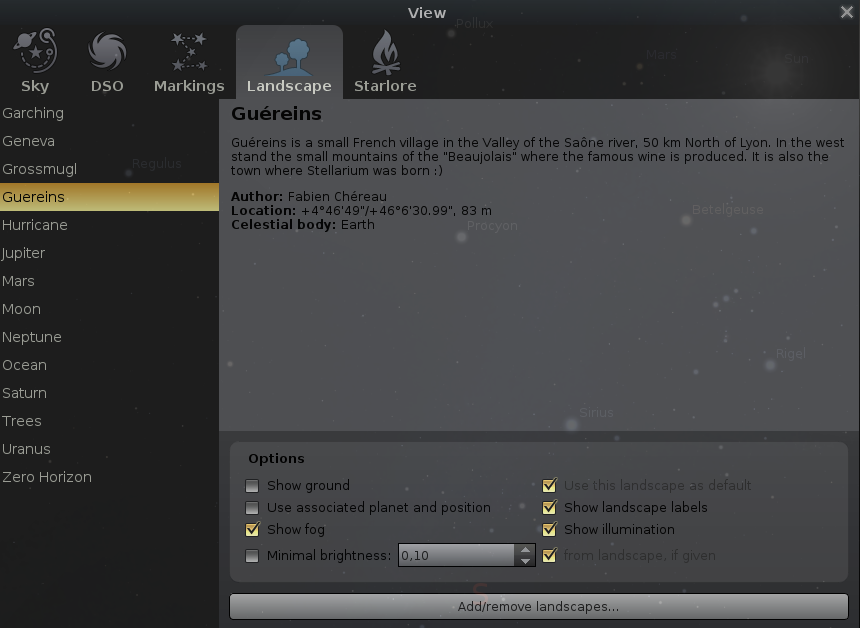
\includegraphics[scale=0.68]{view_dialog_landscape_tab}
%\caption{Figure caption}
\end{figure}

The Landscape tab of the View window controls the landscape graphics
(ground). To change the landscape graphics, select a landscape from the
list on the left side of the window. A description of the landscape will
be shown on the right.

Note that while landscape can include information about where the
landscape graphics were taken (planet, longitude, latitude and
altitude), this location does not have to be the same as the location
selected in the Location window, although you can set up Stellarium such
that selection of a new landscape will alter the location for you.

The controls at the bottom right of the window operate as follows:

\begin{itemize}
\item
  \textbf{Show ground} This turns on and off landscape rendering (same
  as the button in the main tool-bar).
\item
  \textbf{Show\_fog} This turns on and off rendering of a band of
  fog/haze along the horizon.
\item
  \textbf{Use associated planet and position} When enabled, selecting a
  new landscape will automatically update the observer location.
\item
  \textbf{Use this landscape as default} Selecting this option will save
  the landscape into the program configuration file so that the current
  landscape will be the one used when Stellarium starts.
\end{itemize}

\subsubsection{Starlore Tab}\label{starlore-tab}

\begin{figure}[h]
\centering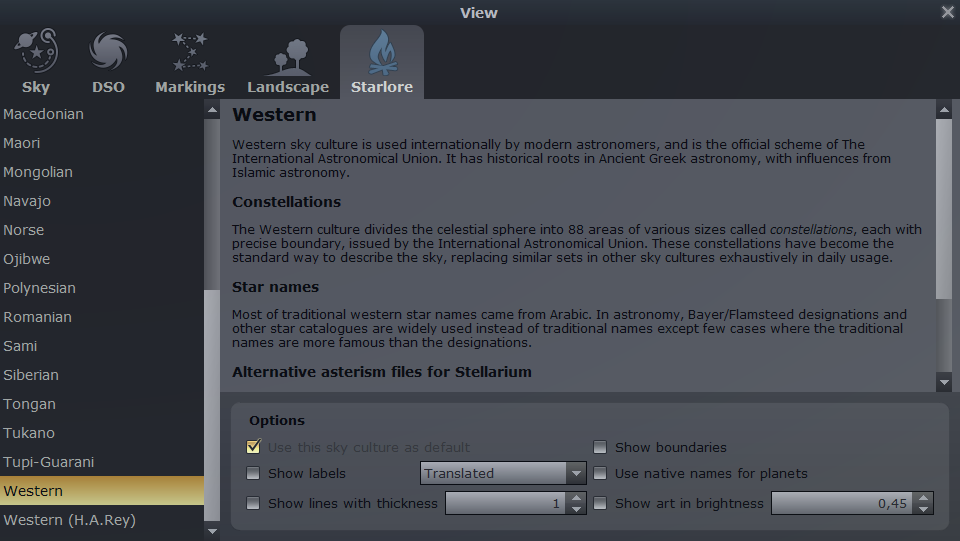
\includegraphics[scale=0.68]{view_dialog_starlore_tab}
%\caption{Figure caption}
\end{figure}

The Starlore tab of the View window controls what culture's
constellations and bright star names will be used in the main display.
Some cultures have constellation art (Western and Inuit), and the rest
do not.
